\chapter{Introducción}
\section{Contexto General}

Dar forma gráfica a la información es una herramienta valiosa, permitiendo que la misma sea más fácil y rápida de entender, comunicar e incluso aprender.

Para contextualizar correctamente el rol de la visualización, es útil distinguir entre los conceptos de \textbf{datos}, \textbf{información} y \textbf{conocimiento}. Los \textit{datos} son registros crudos, sin procesar, que por sí solos no necesariamente transmiten significado. Cuando estos datos se organizan y procesan para responder a una pregunta o cumplir un propósito, se convierten en \textit{información}. Finalmente, cuando esa información se interioriza, se conecta con experiencias previas y permite tomar decisiones, se transforma en \textit{conocimiento}.

Este proceso de transformación es clave en contextos como el análisis de grandes volúmenes de datos, donde la visualización actúa como puente entre la información y el conocimiento: nos ayuda a detectar patrones, comprender relaciones y llegar a conclusiones útiles de manera más eficiente.

Algo tan simple como analizar manualmente los registros de un sistema —lo cual puede requerir una cantidad considerable de tiempo para comprender qué ocurrió en un determinado día o a una hora específica— puede graficarse como una serie de tiempo y permitir que ese análisis se realice en cuestión de segundos.

Todo esto es posible gracias a la \textbf{visualización}, que para efectos de esta Memoria de Título podemos entender como el uso de representaciones visuales interactivas, asistidas por computadora, para ayudar a la cognición~\cite{card1999readings}. 

A pesar de esta definición, que posiciona la visualización como una herramienta que sienta sus bases en la computación, sus orígenes no se alinean con la llegada de la tecnología moderna. El adagio ``Una imagen vale más que mil palabras'', atribuida al dramaturgo y poeta Henrik Johan Ibsen, demuestra cómo esta idea se asienta en el imaginario colectivo como una verdad lógica. Incluso remontándonos a tiempos previos a nuestra era, las civilizaciones tempranas utilizaron distintos métodos para representar datos de forma visual, como el mapa estelar de Suzhou de la dinastía Song en China, que mostraba 1.434 estrellas agrupadas en 280 constelaciones~\cite{bonnetbidaud2009dunhuang}. Este y otros ejemplos históricos nos demuestran el deseo humano de centrar sus esfuerzos en simplificar información compleja en formas comprensibles y accesibles, utilizando representaciones visuales que potencian nuestra capacidad para observar patrones, relaciones y significados que de otro modo pasarían desapercibidos.

Este concepto es aún más prevalente en los tiempos que corren, ya que la llegada de las computadoras y el software ha revolucionado nuestra capacidad de manejar la información. Es gracias a estos avances tecnológicos que podemos analizar grandes volúmenes de datos complejos, que normalmente no podríamos haber procesado sin la aparición de software específico para este objetivo. Nos referiremos a este tipo de datos como \textbf{Macrodatos} o \textbf{Big Data}~\cite{mcafee2012bigdata}.


\subsection{Big Data}

La definición de \textit{Big Data} corresponde a la información de gran volumen, gran velocidad y gran variedad que requiere formas innovadoras y eficientes para su procesamiento. Sin embargo, este término se popularizó alrededor del año 2012~\cite{diebold2012bigdata}, y lo que se consideraba \textit{Big Data} en el pasado es de mucha menor magnitud de lo que se considera hoy en día. Así mismo, la magnitud de estos datos en un futuro será mayor, ya que las capacidades de almacenamiento y procesamiento aumentarán.

Por tanto, se considerarán algunas características esenciales para asegurarnos de que estamos lidiando con macrodatos.
\begin{enumerate}
    \item \textbf{Variedad}:         El conjunto de datos es heterogéneo, y normalmente no posee una estructura concreta para su procesamiento de manera nativa.
    \item \textbf{Velocidad}: 
        Se refiera a la rapidez con la que los datos se generan. Normalmente los tipos de datos a analizar están en tiempo real, y generan nuevos datos a una frecuencia alta.
    \item \textbf{Volumen}: 
        La cantidad de datos es significativa para el sistema donde se está trabajando y la tecnología actual.
\end{enumerate}

Otra característica importante a considerar de esta definición, es que estos datos son \textbf{inútiles} por sí solos,~\cite{gandomi2015beyond} la relevancia de este gran volúmen de información proviene del conjunto de \textbf{todos} los datos y la \textbf{interpretación} de los mismos. 

Al representar visualmente, por ejemplo, una serie de tiempo, es necesario acceder a cada uno de los elementos contenidos en el conjunto de datos para construir la gráfica correspondiente. Supongamos que disponemos de una secuencia de \( n \) puntos ordenados \((x_1, y_1), (x_2, y_2), \ldots, (x_n, y_n)\), los cuales deben ser procesados por el motor de renderizado de la herramienta de visualización. Este proceso conlleva, en el mejor de los casos, una complejidad temporal \(\mathcal{O}(n)\), ya que se requiere al menos una operación por cada punto para construir su representación gráfica.

Este comportamiento lineal implica que el tiempo necesario para renderizar una visualización crece proporcionalmente con la cantidad de datos. Por ejemplo, en la Figura~\ref{add_trace_plotly} se observa cómo la visualización de una serie de aproximadamente 350 mil puntos requiere cerca de 1.5 segundos para ser completada. Este tiempo, aunque aparentemente breve, resulta considerable en escenarios donde se espera interacción fluida, como el análisis exploratorio o los tableros de monitoreo en tiempo real.

\begin{figure}
    \centering
    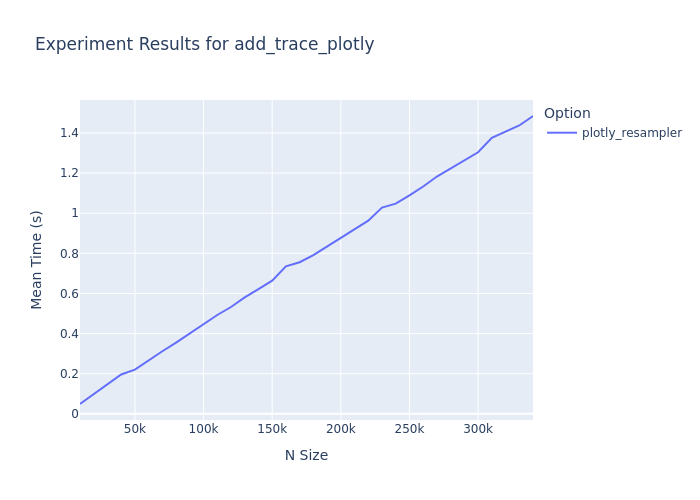
\includegraphics[width=0.9\linewidth]{introduction/images/add_trace_plotly.png}
    \title{figure}
    \caption[Tiempo Renderización Plotly]{Tiempo promedio en segundos de graficar N cantidad de puntos usando la librería plotly.}
    \label{add_trace_plotly}
\end{figure}

De acuerdo con el informe publicado por Visa en 2017~\cite{visa2017facts}, su plataforma global de pagos posee la capacidad de procesar hasta 65{,}000 transacciones por segundo en condiciones de carga máxima. Sin embargo, en escenarios de uso más comunes, el volumen de transacciones tiende a rondar las 2{,}000 por segundo. Si consideramos un análisis retrospectivo de un solo día completo, el volumen total de datos asciende a un intervalo entre aproximadamente \(2{,}000 \times 86{,}400 = 1.728 \times 10^8\) (uso bajo) y \(65{,}000 \times 86{,}400 = 5.616 \times 10^9\) (uso máximo) transacciones por día.

Bajo este escenario, un trabajador que requiera analizar la actividad completa de un solo día enfrentaría una carga de datos que oscila entre cientos de millones y varios miles de millones de registros. Si asumimos un proceso de visualización con complejidad temporal \(\mathcal{O}(n)\), incluso los enfoques más optimizados en términos de eficiencia enfrentarán tiempos de procesamiento significativos y haciendo inviable su análisis oportuno.

Además del rendimiento, cuando trabajamos con series temporales extremadamente densas o con puntos altamente consecutivos entre sí, obtenemos gráficos difíciles de interpretar visualmente. Este problema genera la impresión de gráficos comprimidos o saturados (``quashed"), dificultando enormemente su cognición, como puede observarse claramente en la Figura \ref{squashed_plot}, que representa la lectura de un sensor colocado en un puente.

El creciente volumen de datos en contextos de Big Data nos obliga a repensar los fundamentos mismos de la visualización. Si graficar cientos de miles de puntos ya representa un reto técnico y cognitivo, ¿qué ocurre cuando nos enfrentamos a millones o incluso miles de millones de registros? En estos casos, la visualización deja de ser una simple representación directa de los datos y se transforma en un proceso de síntesis y decisión: ¿qué se debe mostrar, qué se puede omitir, y cómo evitar distorsionar la información en el camino?


\subsection{Downsampling}

Mejorar la eficiencia de los procesos que permiten la visualización es una manera de reducir los tiempos de cómputo, pero existen millones de escenarios donde esto no es suficiente. Aún con estas mejoras, llega una cantidad de puntos que simplemente no es viable visualizar en un tiempo prudente. Así mismo, la legibilidad de los gráficos no se resuelve con estos avances.

Es complejo escapar de esta problemática, ya que no podemos reducir la complejidad temporal lineal a menos que \textbf{no grafiquemos todos los puntos}.

Bajo esa idea surge la técnica conocida como \textit{downsampling}, la cual consiste en seleccionar solo un subconjunto de los puntos originales para ser graficados. A diferencia de métodos que generan nuevos datos mediante agregaciones o promedios, el \textit{downsampling} busca preservar puntos existentes del conjunto original que sean representativos de su comportamiento general. Su objetivo no es reemplazar el análisis detallado, sino facilitar la interpretación visual de grandes volúmenes de datos en contextos donde mostrar todos los puntos no es viable ni útil~\cite{steinarsson2013downsampling}. Esta técnica permite reducir el tiempo de renderizado y evitar la saturación visual sin comprometer, en teoría, la percepción de patrones relevantes. No obstante, su aplicación exige un criterio claro: ¿qué puntos se deben conservar para que la visualización siga siendo fiel a los datos?

Este acercamiento permite mejorar el rendimiento y la legibilidad sin comprometer significativamente la percepción de patrones relevantes. Existen múltiples algoritmos diseñados con este fin, los cuales serán analizados en detalle en la Sección~\ref{alternatives}.

\begin{figure}[H]
    \centering
    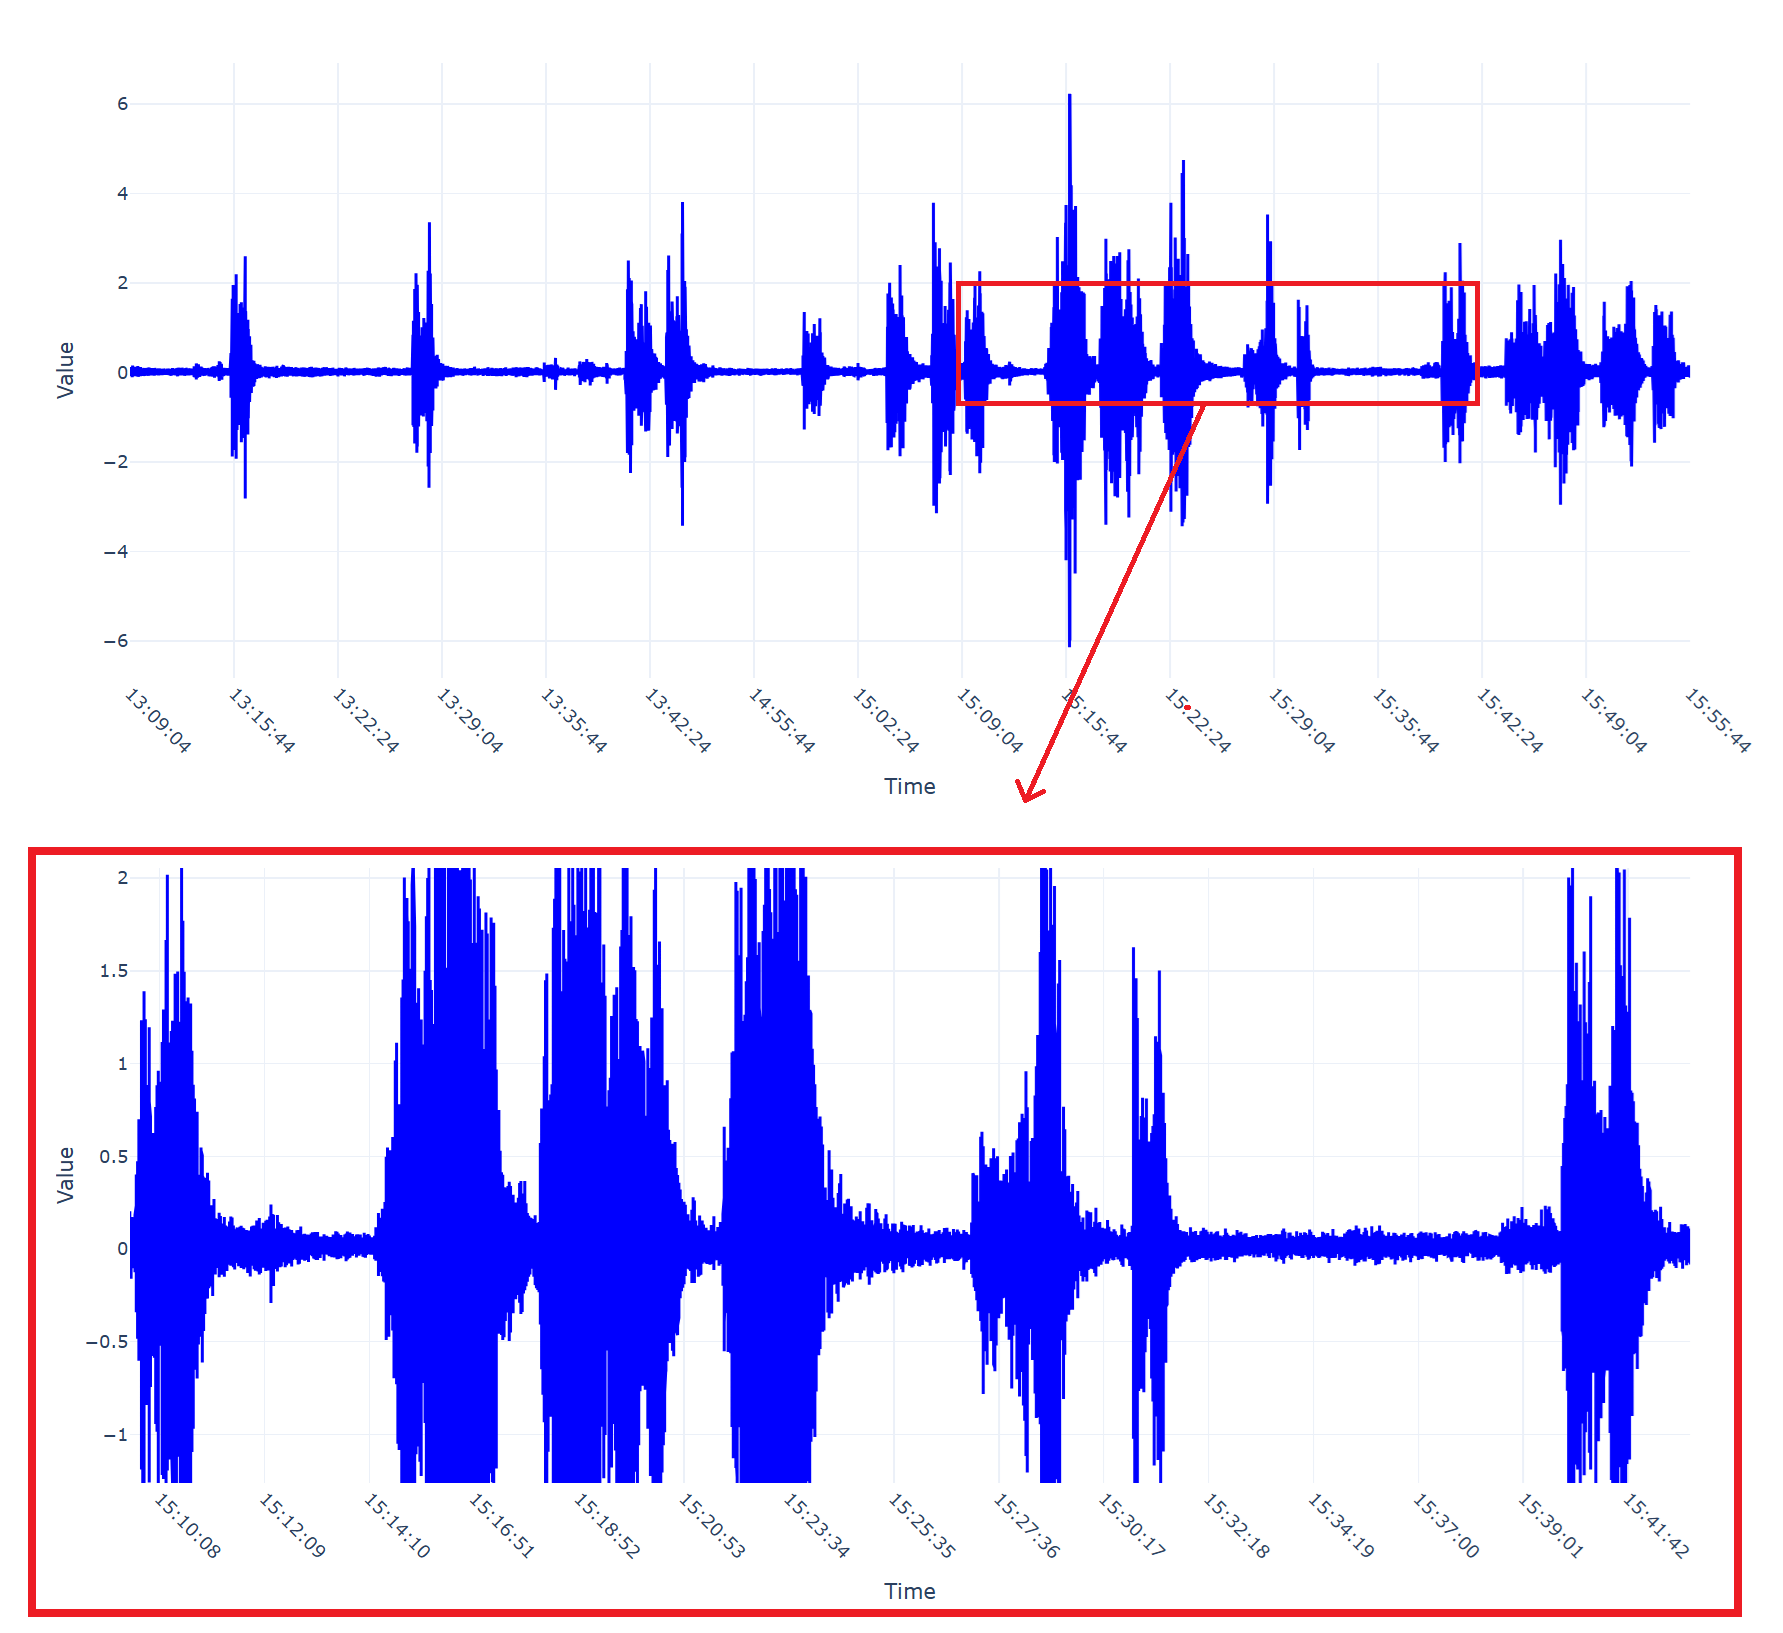
\includegraphics[width=0.9\linewidth]{introduction/images/squashed_plot.png}
    \caption[Serie de Tiempo Sin Downsample]{Serie de tiempo con aproximadamente 350,000 puntos con valores del sensor de un puente. Al ser demasiados puntos por segundo, es difícil identificar el comportamiento del sensor en cada segundo.}
    \label{squashed_plot}
\end{figure}

\begin{figure}[H]
    \centering
    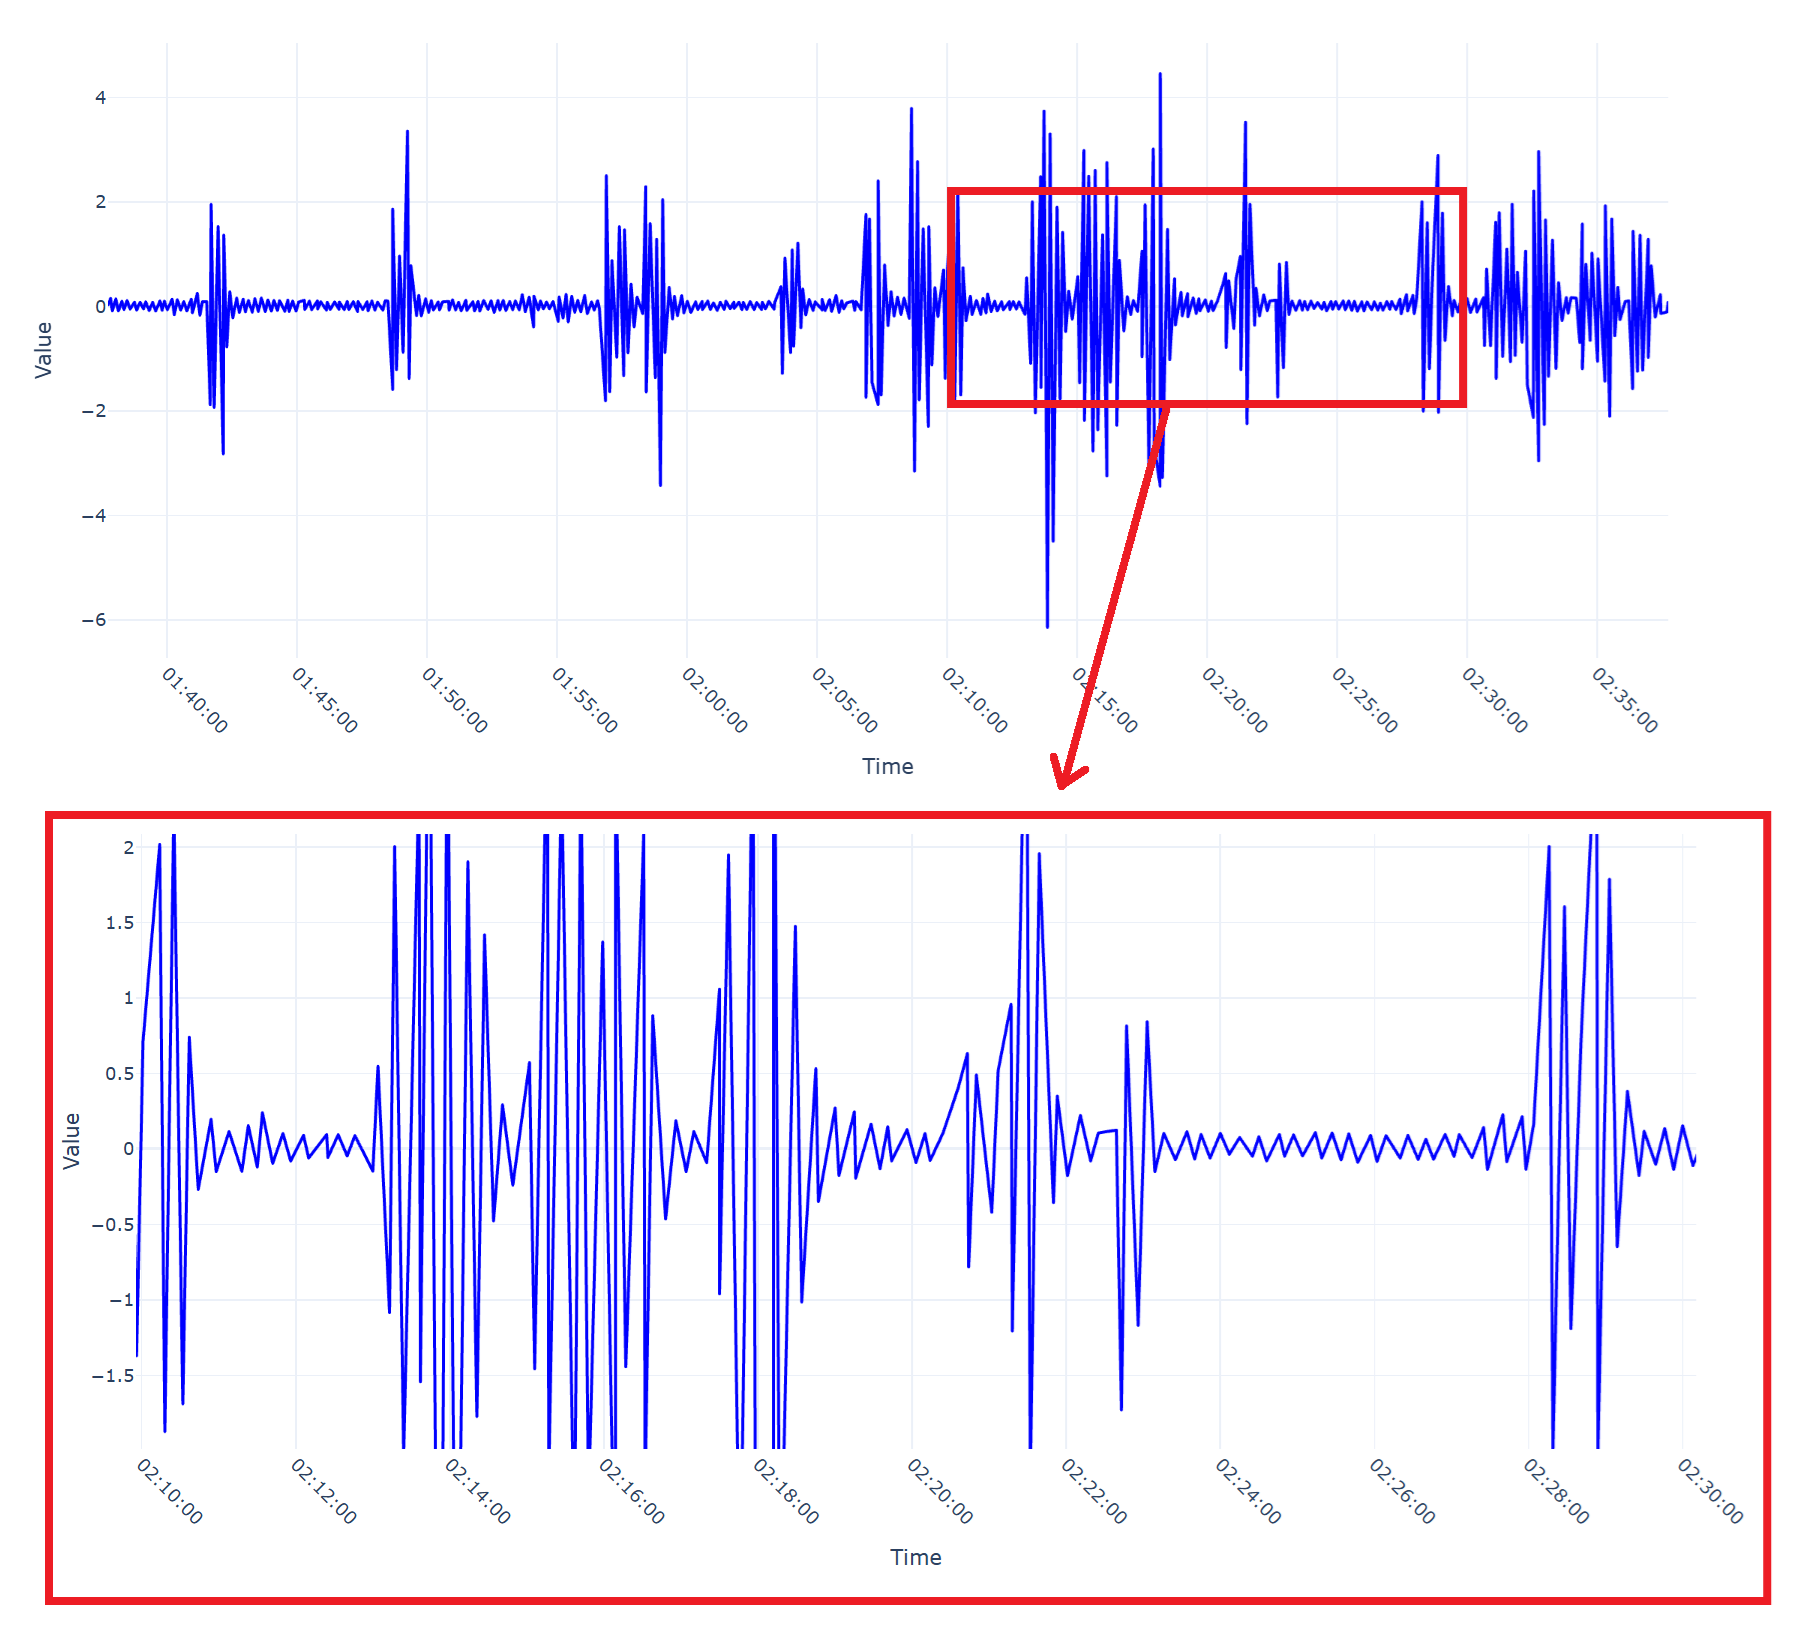
\includegraphics[width=0.9\linewidth]{introduction/images/downsample.png}
    \caption[Serie de Tiempo Con Downsample]{Downsample de serie de tiempo con aproximadamente 350,000 puntos con valores del sensor de un puente.}
    \label{downsample}
\end{figure}

El grupo de investigación \textbf{PreDiCT.IDLab}\cite{predict2025}, afiliado a la Universidad de Gante en Bélgica, ha desarrollado e investigado activamente métodos avanzados para la visualización eficiente de series de tiempo. Entre sus contribuciones destaca la herramienta \texttt{tsdownsample}, un conjunto de algoritmos de alto rendimiento diseñados específicamente para realizar downsampling en contextos de visualización~\cite{tsdownsample}, la cual implementa los algoritmos ya mencionados para ser utilizados en \textit{Python}.

Otra biblioteca de gran utilidad creada por estos académicos es \textit{plotly-resampler}~\cite{plotly-resampler}, la cual integra \textit{tsdownsample} de manera directa en \textit{plotly}. A pesar del preprocesamiento necesario para generar una submuestra de una serie de tiempo, aún así podemos ver diferencias significativas en el tiempo necesario para la visualización de conjuntos grandes de información.

Esta mejora es evidente en la Figura \ref{plotly_vs_resampler}, donde podemos observar cómo usar \textit{plotly-resampler} disminuye el tiempo de renderización del gráfico para un conjunto de pares ordenados, a pesar de que es un \textit{wrapper} de \textit{plotly} y procesa el vector original. 

Esto se debe a que la cantidad de puntos seleccionados para renderizar $(n_{out})$ es fija (por defecto 1000), lo que permite que la renderización final tenga una complejidad constante $\mathcal{O}(n_{out})$, es decir, $\mathcal{O}(1)$ al no depender del tamaño de la serie original. Sin embargo, es importante destacar que el paso previo de downsampling —donde se procesa el conjunto completo de datos de entrada— sí presenta una complejidad lineal $\mathcal{O}(n)$ con respecto al tamaño original de la serie. Por lo tanto, el beneficio radica principalmente en acelerar la renderización e interacción con el gráfico una vez generado.


\begin{figure}[H]
    \centering
    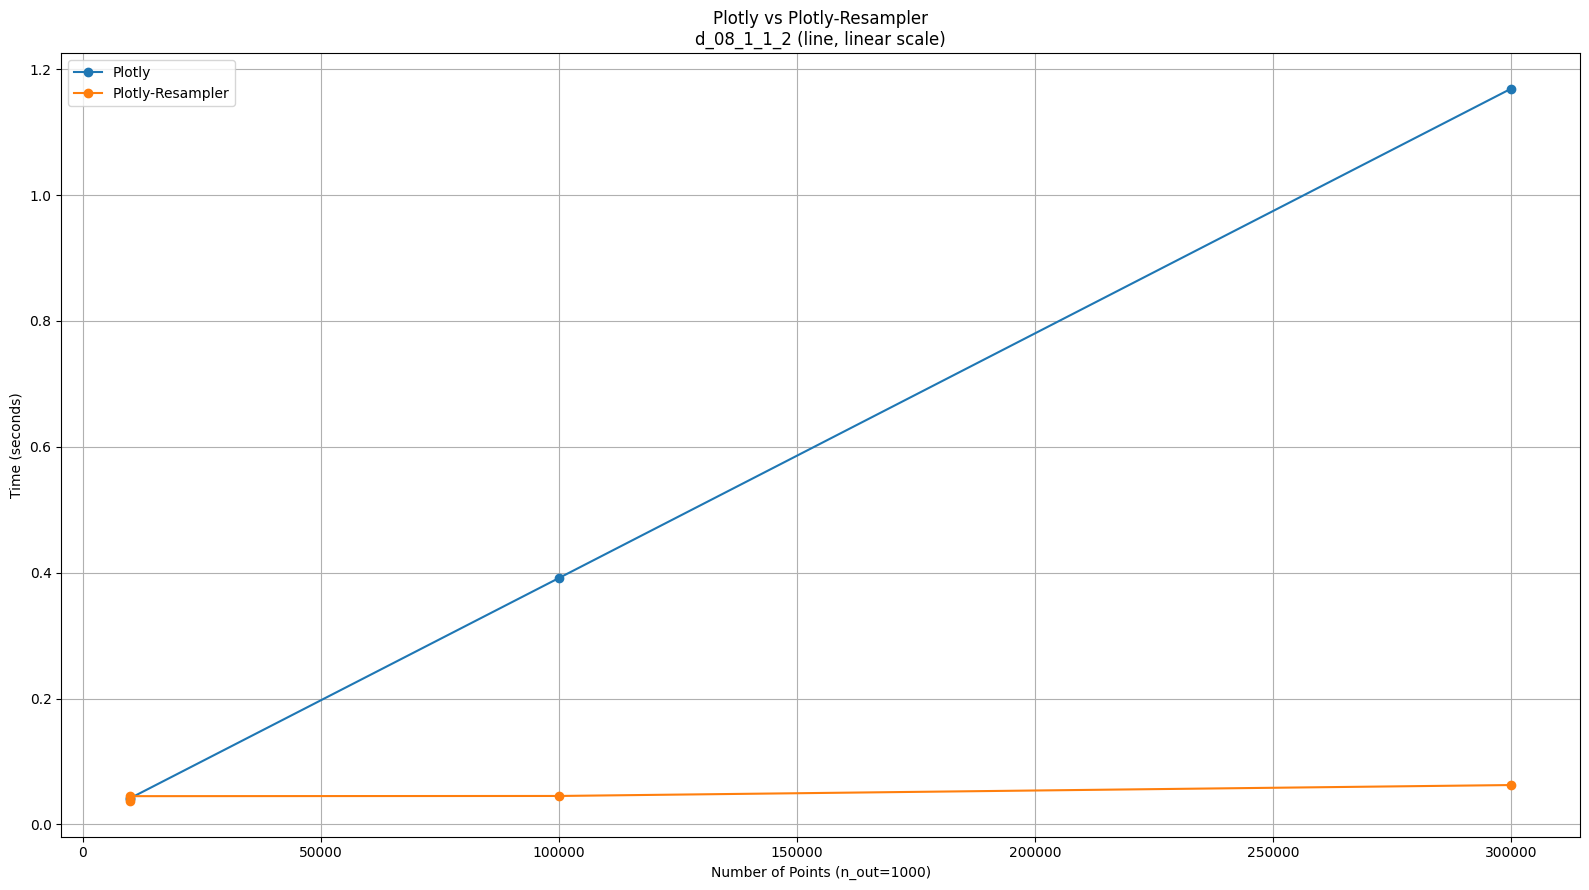
\includegraphics[width=0.9\linewidth]{introduction/images/plotly_resampler.png}
    \caption[Tiempo de Renderizado Plotly vs Plotly-Resampler]{Comparación de tiempo entre las librerias \textit{plotly} y \textit{plotly-resampler} al crear gráficos con $n$ cantidad de puntos.}
    \label{plotly_vs_resampler}
\end{figure}

En definitiva, usar estrategias de \textit{downsample} es una opción muy útil a la hora de visualizar una serie de tiempo con muchos puntos, ya que permite mejorar la legibilidad, tiempo de renderización y, a causa de esto, el análisis de los datos que se están estudiando.

\section{Presentación del Problema}

Las técnicas de \textit{downsampling} han demostrado ser altamente efectivas para mejorar la experiencia de visualización de series de tiempo densas. Al reducir la cantidad de puntos a representar, se agiliza el tiempo de renderizado, se disminuye la sobrecarga cognitiva y se facilita la exploración visual de grandes volúmenes de información.

Sin embargo, el uso de downsampling por sí solo no resuelve todos los desafíos asociados a la visualización eficiente. En particular, el enfoque actual tiende a reemplazar temporalmente los datos originales por una submuestra que se visualiza, dejando de lado tanto el almacenamiento de los datos originales como el manejo eficiente de múltiples niveles de resolución.

Esta Memoria de Título busca ampliar el alcance de dicha problemática proponiendo un enfoque complementario, en el que \textbf{coexistan en memoria tanto los datos originales como sus versiones downsampleadas a diferentes niveles de detalle}. En lugar de recalcular constantemente nuevas submuestras o depender de múltiples archivos, se plantea la posibilidad de mantener todas estas representaciones disponibles simultáneamente.

El principal beneficio de esta idea es que permitiría, por ejemplo, realizar transiciones dinámicas entre distintos niveles de zoom o densidad de puntos durante la visualización, sin necesidad de recargar datos desde disco ni efectuar nuevos cálculos en tiempo real. Si el usuario desea acercarse a una región específica de una serie, podría acceder directamente a una versión más detallada ya presente en memoria; si desea una vista general, se podría utilizar una versión más resumida. Todo esto sería posible dentro del mismo entorno de ejecución, aprovechando la coexistencia de los datos en distintas resoluciones.

Para lograr esta integración sin incurrir en un incremento significativo del espacio ocupado, esta memoria explora el uso de \textbf{estructuras de datos compactas}, capaces de representar información de manera más eficiente que los formatos tradicionales. La intención es que, idealmente, el conjunto completo —datos originales más múltiples niveles de downsampling— pueda almacenarse en una cantidad de memoria comparable a la de los datos originales solos. Por ejemplo, si una serie de tiempo ocupa originalmente 1~GB en memoria, el objetivo sería almacenar en ese mismo espacio no solo la serie completa, sino también varias representaciones resumidas que puedan ser utilizadas directamente para visualización rápida.

Ahora bien, las estructuras de datos compactas que se estudiarán no fueron diseñadas originalmente para tareas de visualización ni para el almacenamiento de números flotantes. Por lo tanto, su aplicabilidad directa a este contexto es bastante limitada. La mayoría están optimizadas para almacenar enteros positivos, lo que impone restricciones adicionales sobre el tipo de datos que pueden manipularse eficientemente.

Por esta razón, esta memoria no busca implementar un sistema completo de visualización multiresolución, sino que se plantea como una \textbf{prueba de concepto}. Se construirá un esquema inicial que permita evaluar en qué medida estas estructuras podrían adaptarse al almacenamiento y visualización de datos numéricos —incluyendo flotantes— utilizando diferentes bibliotecas de visualización. Este trabajo busca sentar las bases para desarrollos futuros en visualización eficiente de series de tiempo utilizando estructuras de datos compactas.
